%
		\subsection{2d3v PIC}\label{sec:pic_2d3v}
%
			In the following, I will highlight the difficult tasks of a spatially twodimensional PIC simulation, refering to the scheme in~\autoref{fig:picscheme}.
%
			\paragraph{Simulation Model}%
			In the beginning of the simulation, before the first calculation step is done, the domain has to be constructed. The cylindrical setup is reduced to the radial and axial dimensions, e.g\@ $(r,z)$ for reasons of symmetry. The five-dimensional phase-space is completed with the full velocity triplet $\vec{v}=(v\ix{r},v\ix{z},v_{\vartheta})$. The two-dimensional mesh expands in radial and axial direction by $N\ix{r}$ and $N\ix{z}$ equally sized partitions respectively. Thus, the area of a single mesh cell is $\Delta r\ix{0}^{2}$. The spatial and temporal discretisation $\Delta r\ix{0}$ and $\Delta t\ix{0}$ are chosen to be dimensionless, so calculations inside the code can be performed much more easily and are less likely to have errors.\\
			Additionally, certain physical properties have to be scaled according to the spatial weight of a cell. Because a `quasi-three-dimensional' cell of coordinates $(n\ix{r},n\ix{z})$ grows in volume with increasing radial index (for a more visual approach, take a look at~\autoref{fig:radialcylinder}), a weighting factor needs to be multiplied with properties like densities and pressure.\\
			Next the particle species have to be initialised. Here, one uses pressure and intial density to model a global distribution of electrons, ion and neutral species. The corresponding super particle factor is used to decrease computational time. Though it has been proven that this does not introduce artifacts to the simulations results --- the equation of motion only depends on a charge-to-mass-ratio --- it should not be too high. Collisions may be underrepresented when there are not enough targets, though in reality $\sim\tenpo{4}$ times the amount of particles would be available.\\
			A number of electrons, ions and neutrals is distributed in each cell, using a Maxwell-distribution-function. Inside one mesh cell the particles are spread random and continuously. The same goes for the velocity, which is randomly picked from the specified distribution function. The radial deformation of each cell has to be taken into account here. Therefore more particles have to be initiated in cells the closer they get to the outer limit of the cylindrical domain.
%
			\paragraph{Potential and Field Calculation}
			After the domain is filled the resulting density distribution, potential and electric field have to be calculated. The charges need to be mapped to the grid points to generate a density, which is used to solve Poisson's equation (see~\autoref{equ:fivepointstar}). A linear weighting function is applied for each charge to form the density. The resulting scheme for a particle at $(r,z)$ in one and two dimensions is shown in~\autoref{fig:cicweighting} and~\autoref{equ:cicweighting}. The index tuple $k,j$ denotes the position in the twodimensional mesh, $n\ix{k,j}$ the corresponding density, $(r\ix{k},z\ix{j})$ the position --- this e.g\@ would be $r\ix{k}=\Delta r\ix{0}\cdot k$ and so on --- and $S\ix{k,j}$ the statistical weight, composed of dimensionless charge, super particle and volume factor. The quotient $A\ix{k,j}=\Delta r\ix{0}^{2}$ normalizes the result, so that no error is made when summarizing all four contributions of a single particle to the density.
%
			\begin{figure}
				\centering
				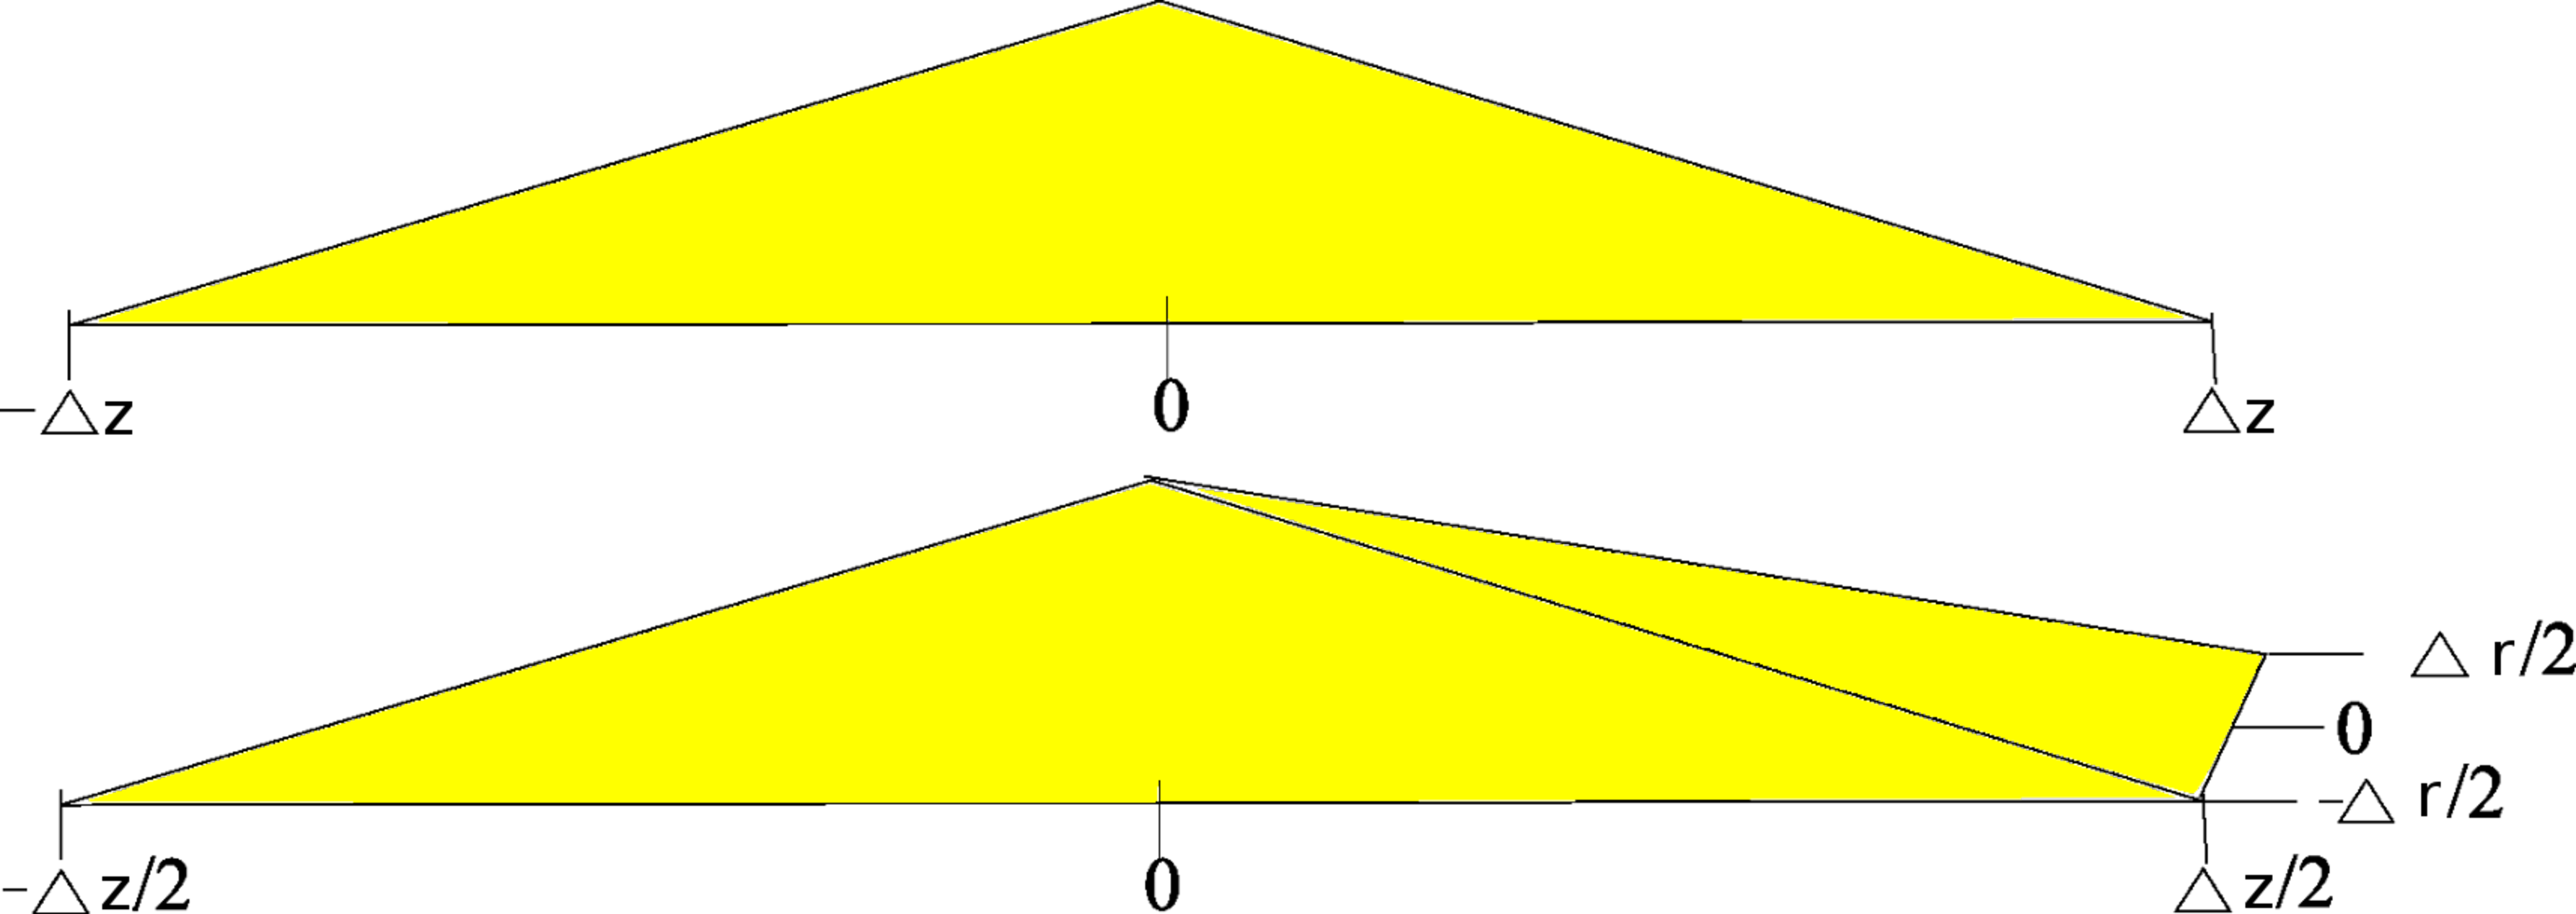
\includegraphics[width=0.8\textwidth]{figures/cicweighting.pdf}
				\caption{%
					Linear weighting scheme for (top) 1D and (bottom) 2D simulations. The latter is an expansion into the radial dimension from a 1D case. The twodimensional approximation is called Cloud-In-Cell (CIC)~\cite{Matthias15}.%
			}\label{fig:cicweighting}
			\end{figure}
%
			\begin{align}
				\text{1D:}\quad\quad\,\,\,\,%
					n\ix{j}&=\frac{S\ix{j}}{\Delta z}\left(z\ix{j}-z\right)%
					\label{equ:cicweighting1d}\\[0.0cm]
				\text{2D:}\quad\quad%
					n\ix{k,j}&=\frac{S\ix{k,j}}{A^{2}\ix{k,j}}%
					\left(r\ix{k+1}-r\right)\cdot\left(z\ix{j+1}-z\right)%
					\label{equ:cicweighting}
			\end{align}
%
			To avoid possible self-forces and satisfy the conservation of momentum, the same weighting method has to be used when back-mapping the calculated forces from the discrete grid points to the particle positions. Again, for a more detailed discussion see~\cite{Tskhakaya}.\\
			The discrete matrix~\autoref{equ:poissonpotential} is solved using a \emph{LU-factorisation}. On the system side this process is optimised by the matrix-solver library~\emph{SuperLU}, which is a program tool for the direct solution of large, sparse non-symmetric systems of linear equations. There are also other matrix-solver algorithms, for example the successive-over-relaxation (SOR) or gradient descent method.\\
			The potential is calculated on every time step using this factorisation, but the latter is done only once at the beginning, because it only depends on the mesh, and hence the composition of the matrix $\Phi\in\mathbb{R}^{N\ix{r}\times N\ix{z}}$. At this is point any potential boundary conditions, such as external voltages $U\ix{rf}(t)$ or ground $\Phi=0$ are applied to the result of $\Phi$.\\
			The calculated force from~\autoref{equ:efieldmaxwell} is again mapped back to the individual particle positions using the same scheme as~\autoref{equ:cicweighting} for the two-dimensional mesh. Therefore, momentum and energy conservation is satisfied.\\
			The resulting field and potential are distributed to all processing cores afterwards. The following routines are exercised on the corresponding domain partitions in parallel, which shares the computational burden and a lot of calculation time.
%
			\paragraph{Particle Pusher}
			The force acting on the particles is used in the $N$ equations of motion from~\autoref{equ:leapfrogscheme}. This method is called \emph{Boris algorithm}. The particle $n$ is pushed, according to the calculated velocity $v\ix{n,k+1/2}$ and previous position $x\ix{n,k}$, to its new position $x\ix{n,k+1}$. We will only consider the movement of charged species. A neutral push is not necessary, because the distribution of the neutral gas reservoir can be considered homogeneous due to their very large mean free path of $\sim\unit[2-30]{cm}$, depending on the pressure.\\
			Because we know that the electrons are the fastest species in the discharge, and the time step is chosen to sufficiently describe all plasma processes, one can significantly save computation time when pushing the slower species less often. Therefore a subcycling routine is written, which pushes the heavier and slower ions only every few steps, e.g\@ 2-6 code cycles. The subcycling factor is sensitive to the species velocities, because the particles should not be pushed further than one Debye length $\lambda\ix{D}$ to avoid numerical problems. The subcycling method is also applied to the collision routine, which again saves more computational time.\\
			After all velocities have been calculated and the particles are pushed, boundary conditions such as secondary emission, reflection and absorption at the walls are applied. Those processes are in general far from trivial. Therefore a \emph{Monte-Carlo} algorithm is used, in which a random generated number $R\in[0,1]$ is compared with the probability $P(\theta,E)$ of a corresponding physical process, e.g.\@ secondary emission. This probability is a function of incident angle $\theta$ and energy $E$. For $P>R$ the secondary particle of species $j$ is injected with a given velocity distribution $f\ix{j}^{sec}(\vec{v})$, other wise the projectile is just lost (see~\autoref{sec:surfaceeffects} and~\autoref{sec:negionphysics}).
%			
			\paragraph{Collision Routines}
			The importance of collisions in ccrf discharges has been discussed earlier in~\autoref{sec:heating} and~\autoref{sec:negiondynamics}. In contrast to a global method, which calculates every single of the $N^{2}$ particle-particle interactions, a binary collision model is used. In this algorithm only particles from the same Debye cell are considered to collide with each other. Because self-forces where excluded from the simulation by the weighting scheme in the previous section, the inter-particle forces inside grid cells are underestimated. This can partially be compensated when introducing Coulomb collisions of charged particles using the binary collision operator. This still satisfies energy and momentum conservation and is sufficiently accurate~\cite{Tskhakaya}. Random pairs of charges are chosen from one cell, so each particle has a single partner. This pair then is statistically collided using the simple approach from above of the boundary conditions.\\
			For charged-neutral collisions the classical \emph{Monte-Carlo-Collisions} simulation method is used: let us assume the collision probability
%
			\begin{align}
				P(t)=1-\exp(-\delta t\ix{c}\cdot\nu\ix{n,j})\,.%
				\label{equ:mccollisions}
			\end{align}
%			
			Here $\nu\ix{n,j}=\sum_{i=1}^{I}\nu\ix{n,j}^{(i)}$ is the collision frequency of neutrals and species $j$, written as the sum of all possible collisions. A single frequency is a function of $\nu^{(i)}=\sigma\ix{i}(v\ix{rel})n\ix{i}$ collision cross-section $\sigma\ix{i}$, density and relative velocity. The value of $\delta t$ is the time between two successive collisions. If $\delta t=t\ix{c}$ the collision time, the probability becomes $P=1$. The minimum collision time is again given by a random generated number $R$
%
            \begin{align}
                t\ix{c}^{min}=-\frac{\ln R}{\nu\ix{n,j}^{max}}\,.%
                \label{equ:collisiontime}
            \end{align}
%
            To further reduce the computational burden, the minimum time between to processes is used to calculate the maximum collision probability for a time step $\Delta t$: $P\ix{max}=1-\exp(-\Delta t\cdot\nu\ix{n,j}^{max})$. Now it is possible estimate the maximum number of colliding particles $N\ix{Coll}=N\cdot P\ix{max}\ll N$. The algorithm now only has to evaluate so many potential collisions and no longer needs to calculate the probability for each individual pair. The selection of the $N\ix{Coll}$ particles is done randomly.\\
            If the condition $R\ge P(t)$ for a particle pair is satisfied the corresponding process is executed. It is not important whether the particles are near each other in the selected Debye cell or their trajectories cross at any point. The collision routine, e.g\@ coulomb scattering or charge exchange are carried out with no respect to particle paths or positions whatsoever.\\
            Coulomb collisions and elastic scattering processes are treated in a center-of-mass-system with isotropic angle distributions for $\chi$ and $\Psi$ of random generated numbers $R\ix{1/2}$.
%
            \begin{align}
                \Psi=2\pi R\ix{1}\,,%
                    \quad\quad%
                    \chi=\sqrt{-2\langle\chi^{2}\rangle\ix{t}\ln R\ix{2}}\,.%
                    \label{equ:scatterangles}
            \end{align}
%
            Afterwards the velocities are transformed back into their original form. This arbitrary collision algorithm is sufficient, because the transport processes and distribution functions are found to be the same as if a physical model would have been used~\cite{Tskhakaya}.\\
            For charge exchange processes the colliding particles are deleted from the memory and new ones are created at the same location respectively, while deriving the corresponding velocities to satisfy the energy and momentum conservation.\\
            At last, the excitation collisions are performed by an elastic scattering algorithm, which subtracts the threshold energy from the projectile before calculating the exit velocities.\\
%
            \newline
            After the solver, particle push, boundary conditions and surface effects have been executed, the only thing left in the PIC cycle are the diagnostics. Those can be e.g.\@ temperature, density, velocities and so on. They can be among the most time consuming parts of the simulation, because great workloads for single core operation may occur.\\
            If the diagnostics have been collected, the algorithm starts again with calculating the plasma properties for the associated particle pusher (see \textbf{Potential and Field Calculation}).